
\documentclass[12pt]{article}
\usepackage{sbc-template}
\usepackage{graphicx,url}
\usepackage{tikz} 
\usetikzlibrary{automata, arrows, positioning}

\usepackage{mathtools}
\usepackage{amssymb}
\usepackage{amsmath}
\usepackage{algorithm}
\usepackage[noend]{algpseudocode}

\usepackage{listings}
\usepackage{xcolor}
\usepackage[utf8]{inputenc}


\makeatletter
\def\BState{\State\hskip-\ALG@thistlm}
\makeatother

\definecolor{codegreen}{rgb}{0,0.6,0}
\definecolor{codegray}{rgb}{0.5,0.5,0.5}
\definecolor{codepurple}{rgb}{0.58,0,0.82}
\definecolor{backcolour}{rgb}{0.95,0.95,0.92}

\lstdefinestyle{mystyle}{
    commentstyle=\color{codegreen},
    keywordstyle=\color{magenta},
    numberstyle=\tiny\color{codegray},
    stringstyle=\color{codepurple},
    basicstyle=\ttfamily\footnotesize,
    breakatwhitespace=false,         
    breaklines=true,                 
    captionpos=b,                    
    keepspaces=true,                 
    numbers=left,                    
    numbersep=5pt,                  
    showspaces=false,                
    showstringspaces=false,
    showtabs=false,                  
    tabsize=2
}

\lstset{style=mystyle}
     
\sloppy

\title{Análise comparativa entre diferentes algoritmo de enumeração de ciclos em um grafo}

\author{Homenique Vieira Martins\inst{1}, Lucas Santiago de Oliveira\inst{2},}

\address{Instituto de Ciências e Informática \\Pontifícia Universidade Católica de Minas Gerais
  (PUC-MG)\\}

\begin{document} 
    \maketitle

    \begin{abstract} 
        This work aims to make a comparative analysis of time between two algorithms,
        in the enumeration of cycles existing in an undirected graph. For this work, 
        a walking and a permutation algorithm were implemented, and the results of the
        same were analyzed in the search for cycles in some graphs of different sizes.
      \end{abstract}
    
      \begin{resumo} 
        Este trabalho tem como objetivo fazer uma análise comparativa de tempo entre dois algoritmos, 
        na enumeração de ciclos existente em um grafo não direcionado. Para esse trabalho foram implementados
        um algoritmo de caminhamento e outro de permutação, e analisados os resultados dos mesmo na busca em de 
        ciclos em alguns grafos de tamanho diversos.
      \end{resumo}
    
    \section{Explicando a classe grafos} \label{sec:graph}
      \paragraph{}A classe grafo que escrevemos é um simples modelo que liga dois pares em C++,
        o primeiro valor é um número inteiro o segundo valor é um par de inteiros. 
        Sendo o primeiro valor o peso das arestas, o próximo é um par de inteiros que
        representam a ligação entre os vértices.

        \begin{lstlisting}[language=c++]
        std::vector<std::pair<int, std::pair<int, int>>> arestas;
        \end{lstlisting}


        \section{Explicando o algoritmo de Kruskal} \label{sec:Kruskal}
        \paragraph{} A ideia da implementação do algoritmo de Kruskal é primeiramente ordenar 
         todos os pesos de arestas e ir ligando eles a partir de Disjoint Sets. Disjoint sets 
         (ou em português União-Busca), é uma estrutura matemática em que grupos não possuem
         elementos que se intersectam, ou seja, não possuem elementos iguais entre eles. Dessa forma,
         é possível se deslocar dentro dessa estrutura em C++ de forma simples e descobrir se algum 
         elemento está em ambas e se estiver, não conectar no grafo final. Resultado em uma MST, 
         a partir de um algoritmo simples.
     

     \section{Explicando a função de Benchmark} \label{sec:benckmark}

     Para a execução do benchmark deve levar em consideração que existem outros processos 
     concorrente que disputar a disponibilidade do processador e por isso a execução de somente um teste pode
      não trazer o custo real de uma operação, pois por um azar a trend que que ficou responsável por rodar o 
      programa já estava ocupada com outro processo e desta forma impactaria negativamente no resultado,para
       mitigar esse problema definido que seria executado $10^5$ de um mesmo algoritmo  com uma configuração de 
       grafo, todo esse tempo e somando a uma variável e após isso é feito uma média do tempo de execução. 
       O que traria um resultado mais preciso do tempo médio de execução,também para um comparativo de dados 
       peguei o maior e menor tempo de execução de um algoritmo em cima de um grafo. 
        
       \section{Apresentação dos valores} \label{sec:resultados}
   
 
       \subsection{Grafo 1}

       \begin{figure}[ht]
         \centering
         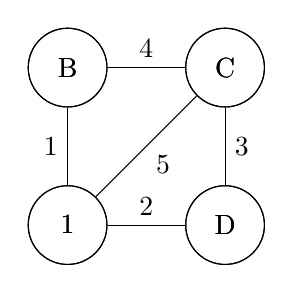
\begin{tikzpicture}[node distance = 3cm,  auto,main/.style = {draw, circle,minimum size=10mm}] 
           \node[main] (1) at (0,0) {1}; 
           \node[main] (2) at (0,2)  {B}; 
           \node[main] (3) at (2,2)  {C};
           \node[main] (4) at (2,0)  {D};
           \node[main] (1) at (0,0)   {1}; 
           \node[main] (2) at (0,2)  {B}; 
           \node[main] (3) at (2,2)  {C};
           \node[main] (4) at (2,0)  {D};
     
           \path[-]
           (1) edge              node {1} (2)            
           (2) edge              node {4} (3)
           (3) edge              node {3} (4)
           (3) edge              node {5} (1)
           (1) edge              node {2} (4);
         \end{tikzpicture} 
         \caption{Grafo \arabic{subsection} - 4 vértices e 5 arestas }
     
       \end{figure}
 


\end{document}